% !TEX root = ../zeth-protocol-specification.tex

\section{\zeth~statement after primitive instantiation}\label{instantiation:statement}

After instantiating the various primitives and providing security proofs to justify that they comply with the security requirements listed in previous sections, $\RELCIRC$ now becomes:

\begin{itemize}
    \item For each $i \in [\jsin]$:
    \begin{enumerate}
        \item $ \auxinputs.\jsins{i}.\znote.\apk = \blake{2s}{\taggedaddr \concat \pad{0}{\blakeCompLen}}$ \\ with $\taggedaddr$ defined in~\cref{instantiation:prf-comm-crh:prf}
        \item $\auxinputs.\jsins{i}.\nf{} = \blake{2s}{\taggednf \concat \auxinputs.\jsins{i}.\znote.\rho}$ \\ with $\taggednf$ defined in~\cref{instantiation:prf-comm-crh:prf}
        \item $\auxinputs.\jsins{i}.\cm{} = \blake{2s}{\auxinputs.\jsins{i}.\znote.\noter{} \concat \msg}$ \\ with $\msg = \auxinputs.\jsins{i}.\znote.\apk \concat \auxinputs.\jsins{i}.\znote.\rrho \concat \auxinputs.\jsins{i}.\znote.\notev$
        \item $\auxinputs.\htags{i} = \blake{2s}{ \taggedpk \concat \priminputs.\hsig}$ (malleability fix, see~\cref{appendix:trnm}) with $\taggedpk$ defined in~\cref{instantiation:prf-comm-crh:prf}
        \item $(\auxinputs.\jsins{i}.\znote.\notev) \cdot (1 - e) = 0$ is satisfied for the boolean value $e$ set such that if $\auxinputs.\jsins{i}.\znote.\notev > 0$ then $e = 1$.
        \item The Merkle root $\mkroot'$ obtained after checking the Merkle authentication path $\auxinputs.\jsins{i}.\mkpath$ of commitment $\auxinputs.\jsins{i}.\cm{}$, with $\mimcSevenMPPrime{}$, equals to $\priminputs.\mkroot$ if $e = 1$.
        \item $\priminputs.\nfs{i}$ \\ $= \indexedset{\pack{\slice{\auxinputs.\jsins{i}.\nf{}}{k \cdot \bnFieldBitCap}{(k+1) \cdot \bnFieldBitCap}}{\FFx{\rBN}}}{k \in [\floor{\prfNfOutLen/\bnFieldBitCap}]}$
        \item $\priminputs.\htags{i}$ \\ $= \indexedset{\pack{\slice{\auxinputs.\htags{i}}{k \cdot \bnFieldBitCap}{(k+1) \cdot \bnFieldBitCap}}{\FFx{\rBN}}}{k \in [\floor{\prfPkOutLen/\bnFieldBitCap}]}$
    \end{enumerate}
    \item For each $j \in [\jsout]$:
    \begin{enumerate}
        \item $\auxinputs.\znotes{j}.\rrho = \blake{2s}{ \taggedrho \concat \priminputs.\hsig}$ (malleability fix, see~\cref{appendix:trnm}) with $\taggedrho$ defined in~\cref{instantiation:prf-comm-crh:prf}
        \item $\priminputs.\cms{j} = \blake{2s}{\auxinputs.\znotes{j}.\noter{} \concat \msg }$ \\ with $\msg = \auxinputs.\znotes{j}.\apk \concat \auxinputs.\znotes{j}.\rrho \concat \auxinputs.\znotes{j}.\notev$
    \end{enumerate}
    \item $\priminputs.\hsig = \indexedset{\pack{\slice{\auxinputs.\hsig}{k \cdot \bnFieldBitCap}{(k+1) \cdot \bnFieldBitCap}}{\FFx{\rBN}}}{k \in [\floor{\crhhsigOutLen/\bnFieldBitCap}]}$
    \item $\priminputs.\resbits = \packResBits{\indexedset{\auxinputs.\jsins{i}.\nf{}}{i \in [\jsin]}, \auxinputs.\vin, \auxinputs.\vout, \auxinputs.\hsig, \indexedset{\auxinputs.\htags{i}}{i \in [\jsin]}}$
    \item Check that the ``\gls{joinsplit} is balanced'', i.e.~check that the \gls{joinsplit-eq} holds:
    \begin{align*}
        &\pack{\auxinputs.\vin}{\FFx{\rBN}} + \sum_{i \in [\jsin]} \pack{\auxinputs.\jsins{i}.\znote.\notev}{\FFx{\rBN}} \\
        & = \sum_{j \in [\jsout]} \pack{\auxinputs.\znotes{j}.\notev}{\FFx{\rBN}} + \pack{\auxinputs.\vout}{\FFx{\rBN}}
    \end{align*}
\end{itemize}

\begin{remark}
    For higher security, we could use \blake{2b}{} with 32-byte output instead of \sha{256}. In fact, since a precompiled contract computing the \blake{2}{}~compression function~\cite{blakecompietf} has been added to the Istanbul release of \ethereum~(EIP 152~\cite{blake-eip}), it could be possible to write a small wrapper on the smart contracts, in order to hash with \blake{2b}{} with any parameter.
\end{remark}

\subsection{Instantiating the packing functions}\label{instantiation:statement:pack}

As we consider SNARKs based on arithmetic circuits defined over a prime field, all variables in the constraint system are interpreted as field elements. Nevertheless, as illustrated~\cref{zeth-protocol:statement}, part of the statement consists in computing functions which co-domains are sets of binary strings (which may be longer than the bit representation of elements of the finite field). While a bit (i.e.~$\{0, 1\}$) is an element of $\FF_p$ ($p$ prime), it is important to minimize the number of gates in the arithmetic circuit for better performance for the proof generation and minimize the number of input wires to improve the verification time. This can be done by ``packing'' binary strings into a set of field elements by interpreting the binary sequence as the elements' base 2 decomposition. On the one hand, converting binary strings into field elements requires to extend the statement proven by the prover, and thus requires the addition of a few arithmetic gates. On the other hand, doing so allows to minimize the number of primary inputs, which, in fine, reduces the complexity of the SNARK verification carried out on-chain.
Indeed, the cost of $\groth$ zk-SNARK~\cite{groth2016size} proof verification is linear in the number of primary inputs since each input acts as a scalar in a costly scalar multiplication of an element in $\gset_1$. Hence, while packing puts ``(slightly) more pressure'' on the prover -- by adding constraints in the circuit -- it simplifies the verifier's work.

We detail in this section the method by which we encode (resp.~decode) a set of binary strings (resp.~field elements) into a set of field elements (resp.~binary strings). In the rest of this section, the notion of \emph{packing policy} is used to refer to the set of \emph{packing} and \emph{unpacking} functions.

The set of primary inputs is composed of the input nullifiers, the output commitments, the public values (see~\cite[Section 3.4.3]{zethpaper}) along with the signature hash and the authentication tags for security (malleability fix, see~\cref{appendix:trnm}). The complete description of the public inputs is represented in~\cref{instantiation:eq:primary-inputs}.
%
\begin{equation}\label{instantiation:eq:primary-inputs}
    (\indexedset{\priminputs.\nf{i}}{i \in [\jsin]}, \indexedset{\priminputs.\cms{j}}{j \in [\jsout]}, \vin, \vout, \hsig, \indexedset{\priminputs.\htags{i}}{i \in [\jsin]})
\end{equation}

Consider the subset of primary inputs that are binary strings, that is the nullifiers $\nfs{}$, the public values $\vin$ and $\vout$, the signature hash $\hsig$ and the authentication tags $\htags{}$.
For each element $x$ in this subset, $\alpha_x = \ceil {\len{x} / \bnFieldBitCap}$, represent the number of field elements to encode all of the element's bits. Let $\beta_x = \floor{\len{x} / \bnFieldBitCap}$ represent the number of field elements which are fully ``filled'' and let $\gamma_x = \len{x} \pmod{\bnFieldBitCap}$ denote the number of remaining bits. For simplicity, as we assume $\zvalueLen < \bnFieldBitCap$, we only define the notation $\gamma_\notev = \zvalueLen$ for the public values $\vin$ and $\vout$.

\begin{example}\label{instantiation:eg:packing}
    Let $\FF'$ be a prime field which elements are encoded on $5$ bits.
%
    If we take a binary string $A \in \bin^7$, such that: $A = (1111011)$, we get: $\alpha_A = 2,\ \beta_A = 1,\ \gamma_A = 2$.
    We illustrate the result of packing $A$ to field elements~\cref{instantiation:fig:packingA}
\end{example}

\begin{figure}[ht]
    \centering
    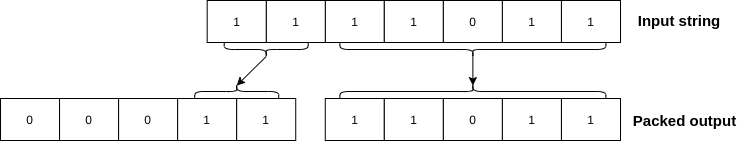
\includegraphics[width=1\textwidth]{images/bit-packing-stringA.png}
    \caption{Packing of string $A$ (see~\cref{instantiation:eg:packing})}\label{instantiation:fig:packingA}
\end{figure}

We denote by $\resBitsBLen$ the total number of bits which could not fully fill a field element, i.e. the weighted sum of the $\gamma_x$,
\[
    \resBitsBLen = \gamma_\hsig + 2 \cdot \gamma_\notev + \jsin \cdot (\gamma_{\nf{}} + \gamma_{\htag{}} )
\]

A simple packing strategy would have been to encode each primary input's field $x$ as $\alpha_x$ field elements. However, this leads to a potentially large waste of space when the PRFs and hash digests are slightly longer than $\bnFieldBitCap$ bits (see~\cref{instantiation:fig:packing-multi-strings}). Another strategy would have been to encode the binary string which results from the concatenation of all binary variables. Doing so, however, would make it expensive to carry out the \emph{unpack} procedure (i.e.~retrieve the original binary strings from the set of field elements, see~\cref{zeth-protocol:process-tx}) on-chain. We thus decided to keep the fully filled $\sum_x \beta_x$ field elements which are ``fully'' filled and aggregate the remaining $\resBitsBLen$ ``residual'' bits in a new variable $\resbits$:
\begin{align*}
    \nfFLen &= \floor{\prfNfOutLen / \bnFieldBitCap} \\
    \hsigFLen &= \floor{\crhhsigOutLen / \bnFieldBitCap} \\
    \htagFLen &= \floor{\prfPkOutLen / \bnFieldBitCap} \\
    \resBitsFLen &= \ceil{\resBitsBLen / \bnFieldBitCap}
\end{align*}

\begin{figure}[ht]
    \centering
    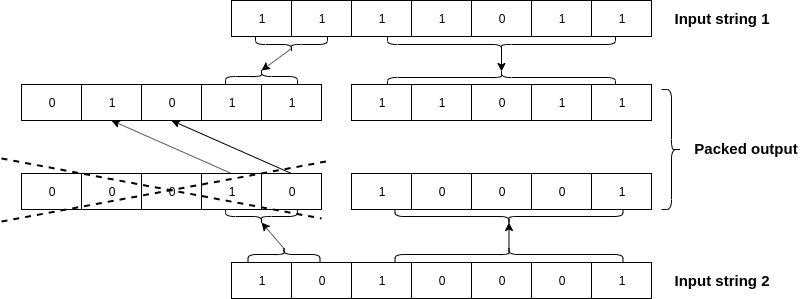
\includegraphics[width=1\textwidth]{images/bit-packing-multi-strings.png}
    \caption{Packing of multiple strings. Observe that, by carefully arranging the bits of the input strings, it is possible to output fewer field elements}\label{instantiation:fig:packing-multi-strings}
\end{figure}

To facilitate the unpacking of the primary inputs, we chose to first aggregate the primary inputs' singular elements. More precisely, regardless of the values $\jsin$ and $\jsout$, the public values $\vin$ and $\vout$, and the hash signature $\hsig$ will always be at the same location in the $\resbits$ string. The residual bits $\resbits$ are thus formatted as follows,
\[
    \vin \concat \vout \concat \widetilde{\hsig} \concat \widetilde{\nfs{}} \concat \widetilde{\htags{}}
\]
where $\widetilde{\hsig}, \widetilde{\nfs{}}, \widetilde{\htags{}}$ are, respectively, the $\gamma_\hsig, \gamma_\nf{}, \gamma_\htag{}$ bits remaining after packing the inputs into field elements.

To format the unpacked primary inputs into field elements, we define the following functions.
The algorithm \pack{}{} (see~\cref{zeth-protocol:fig:packing-alg}), given a bit string of length less than $\bnFieldBitCap$, returns a field element. The algorithm \packResBits{}{} (see~\cref{zeth-protocol:fig:packing-resbits-alg}) given the nullifiers, public values and authentication tags outputs the residual bits. For a given field, the algorithm \unpack{}{}, given the associated packed field elements and the residual bits returns the variables reassembled in binary strings. For instance, we have that $\unpack{\priminputs.\nfs{}, \resbits}{\nf{}} = \indexedset{\auxinputs.\jsins{i}.\nf{}}{i \in [\jsin]}$.
\begin{align*}
    &\pack{}{\FFx{\rBN}} : \BB^{\leq \bnFieldBitCap} \to \FFx{\rBN} \\
    &\packResBits{} : {(\BB^\prfNfOutLen)}^{\jsin} \times {(\BB^\zvalueLen)}^2 \times \BB^\crhhsigOutLen \times {(\BB^\prfPkOutLen)}^{\jsin} \to (\FFx{\rBN})^\resBitsFLen \\
    &\unpack{}{} : \FFx{\rBN}^* \times (\FFx{\rBN})^{\resBitsFLen} \to \BB^* \\
\end{align*}

More particularly, we use the function $\unpack{}{}$ for the nullifiers, public values and signature hash. As such, we have,
\begin{align*}
    &\unpack{}{}_{\hsig} : (\FFx{\rBN})^\hsigFLen \times (\FFx{\rBN})^{\resBitsFLen} \to \BB^\crhhsigOutLen \\
    &\unpack{}{}_{\nf{}} : (\FFx{\rBN})^\nfFLen \times (\FFx{\rBN})^{\resBitsFLen} \to \BB^\prfNfOutLen \\
    &\unpack{}{}_{\vin} : \FFx{\rBN}^0 \times (\FFx{\rBN})^{\resBitsFLen} \to \BB^\zvalueLen \\
    &\unpack{}{}_{\vout} : \FFx{\rBN}^0 \times (\FFx{\rBN})^{\resBitsFLen} \to \BB^\zvalueLen
\end{align*}

\begin{figure*}
    \begin{minipage}[t]{.4\textwidth}
        \centering
        \procedure{\pack{x}{\FFx{\rBN}}}{%
            out \gets 0_{\FFx{\rBN}}; \\
            \pcfor i \in [\len{x}] \pcdo: \\
            \t \pcif x[i] = 1 \pcdo: \\
            \t \t out \gets out +_{\FFx{\rBN}} 2^{\len{x}-1-i} \\
            \pcreturn out;
        }
        \caption{Packing algorithm in big endian.}\label{zeth-protocol:fig:packing-alg}
    \end{minipage}%
    \begin{minipage}[t]{.6\textwidth}
        \centering
        \procedure{\packResBits{\nfs{}, \vin, \vout, \hsig, \htags{}}}{%
            out \gets []; r \gets \epsilon; \\
            r \gets \slice{\vin}{\floor{\zvalueLen / \bnFieldBitCap} \cdot \bnFieldBitCap}{}; \\
            r \gets r \concat \slice{\vout}{\floor{\zvalueLen / \bnFieldBitCap} \cdot \bnFieldBitCap}{}; \\
            r \gets r \concat \slice{\hsig}{\floor{\crhhsigOutLen / \bnFieldBitCap} \cdot \bnFieldBitCap}{}; \\
            %
            \pcfor i \in [\jsin] \pcdo:\\
            \t r \gets r \concat \slice{\nfs{i}}{\floor{\prfNfOutLen / \bnFieldBitCap} \cdot \bnFieldBitCap}{}; \\
            %
            \pcfor i \in [\jsin] \pcdo:\\
            \t r \gets r \concat \slice{\htags{i}}{\floor{\prfPkOutLen / \bnFieldBitCap} \cdot \bnFieldBitCap}{}; \\
            %
            \pcfor i \in [ \ceil{\len{r}/ \bnFieldBitCap} ] \pcdo: \\
            \t out \gets \pack{\slice{r}{i \cdot \bnFieldBitCap}{ (i+1) \cdot \bnFieldBitCap}}{\FFx{\rBN}}; \\
            \pcreturn out;
        }
        \caption{Packing residual bits algorithm.}\label{zeth-protocol:fig:packing-resbits-alg}
    \end{minipage}
\end{figure*}

\subsubsection{Packing Policy Security}
\begin{proposition}[Packing security]
    For a variable $x$ it holds $\unpack{\pack{x}{}}{} = x$ and 
    $\unpack{\packResBits{x}}{} = x$.
\end{proposition}

\subsubsection{Packing Policy Example}

In the case where $\jsin=\jsout=2$, $\bnFieldBitCap$ and all PRFs, and $\crhhsig{}$ output 256 bits, the unpacked primary inputs are 2167-bit long. The packing parameters thus are,
\begin{align*}
    & \resBitsBLen = 143 \\
    & \nfFLen = \hsigFLen = \htagFLen = \resBitsFLen = 1
\end{align*}
The packed primary inputs are 2277 bits long which corresponds to a small space overhead ($\approx 5\%$ unused bits). Moreover, as the residual bits are 143-bit long, they can be written over a single field element. As such, the primary inputs are 9-field element long.
Finally, the residual bits are formatted as follows,
\[
    \underbrace{padding}_{\text{113 bits}} \concat \underbrace{\vin\vphantom{g}}_{64\ bits} \concat \underbrace{\vout\vphantom{g}}_{64\ bits} \concat \underbrace{\hsig}_{3\ bits} \concat \underbrace{\nf{0}}_{3\ bits} \concat \underbrace{\nf{1}}_{3\ bits} \concat \underbrace{\htag{0}}_{3\ bits} \concat \underbrace{\htag{1}}_{3\ bits}
\]
